\section{Experiments}\label{sec:exp}

We ask four questions. (1) How well does one set of weights serve hundreds of heterogeneous
skeletons on text-conditioned generation (\S\ref{sec:exp:main})? (2) How far does the model
extend to a rig it has never seen, with no training and with about ten clips
(\S\ref{sec:exp:extend})? (3) Which capabilities does it combine that released
systems provide separately, and what does the released arbitrary-topology model produce on the same rigs
(\S\ref{sec:exp:compare})? (4) Which ingredients matter
(\S\ref{sec:exp:ablation})?

\subsection{Setup}\label{sec:exp:setup}

\paragraph{Library and splits.} The training library is the \num{311}-rig animal corpus of
\S\ref{sec:method:rep} (\num{77{,}894} clips, \num{6.18}M frames at 30\,fps, 34--102 joints).
Validation holds \num{3{,}899} clips over \num{311} rigs (\num{5}\% of every rig's clips, drawn by a
one seeded permutation per rig; App.~\ref{app:split}). For rigs outside the library we use the
Truebones zoo~\citep{truebones}: \num{986} clips over \num{66} rigs after conversion to \rep{}
with the same pipeline (\num{802} of them carry a caption). Each Truebones rig is split
$80/20$ into train and validation clips by source animation, so that a clip and its cut
neighbours never straddle the split.

\paragraph{Models.} The main model has \num{303}M parameters (14 blocks, width 896, 14 heads);
a \num{36}M pilot (8 blocks, width 384, 6 heads) shares every other setting and is used for
ablations. Both train at global batch 128 with the calibrated objective, the main model for
\num{290} epochs at $1.5{\times}10^{-4}$ and the pilot for 400 at $2{\times}10^{-4}$, with a
4{,}000-step warm-up and a half-cosine decay over 40 epochs to $1\%$ of the peak.

\paragraph{Protocol.} Generation uses 20 Euler steps and text guidance $s{=}2$ everywhere
(\S\ref{sec:method:sampling}); each clip is generated at the length of the real clip, capped at
240 frames, with one seed. Retrieval metrics follow \S\ref{sec:method:eval}: text-to-motion
R-precision at $K{=}1,2,3$ in pools of 64 formed by chunking the dataset order (a retrieved motion
is correct if it is the caption's clip, another export of the same source motion, or a clip with an
identical caption), the FID on the evaluator's
$\ell_2$-normalised embeddings, and the text--motion matching score, each next to the evaluator's
score on the real clips of the same pools (a reference, not a bound). Because a skeleton-aware evaluator exists
only for the library rigs, the Truebones experiments are scored geometrically, in world space,
on the deployable output (the forward kinematics of the predicted rotations): the articulation ratio (mean joint speed relative to the root,
divided by the real clips' value), the jitter ratio (mean second temporal difference, likewise
normalised) and the root speed ratio. Ratios are taken against \emph{all} real clips of the rig at a common 20\,Hz, so that AnyTop samples
and ours are measured identically. The \emph{FK--pose gap} is the mean distance, in the rig's
mean bone length, between the joint positions obtained by forward kinematics of the predicted
rotations and the directly predicted ones: a consistency of the two channels, not a distance to the
target, read from the training-time validation pass (App.~\ref{app:calib}). Library clips are
generated at the real clip's length (at most 240 frames)
from the epoch-289 checkpoint with seed 42; the Truebones arms of \S\ref{sec:exp:extend} use the
epoch-214 snapshot that initialised the adapters, seed 7.

\subsection{One model for 311 skeletons}\label{sec:exp:main}

Table~\ref{tab:main} reports text-to-motion retrieval on the validation set. All \num{311} rigs appear in
training, so this measures the generation of held-out clips on known rigs; rigs outside the library are
the subject of \S\ref{sec:exp:extend}. The \num{303}M
model reaches R@1 \num{0.922} against \num{0.964} for the real clips scored by the same evaluator
in the same pools, a text--motion matching score of \num{0.764} against \num{0.782}, and an FID of
\num{0.005}; the \num{36}M pilot, trained on the same data with the same recipe, reaches R@1
\num{0.897} and FID \num{0.008}. The pools follow the dataset order, so a pool holds clips of one
rig or of neighbouring rigs; R-precision uses the \num{3{,}840} clips of the 60 complete pools, the
matching score and the FID all \num{3{,}899}. The 95\% bootstrap interval over pools is
$[\num{0.907}, \num{0.936}]$ for the \num{303}M R@1 and $[\num{0.955}, \num{0.971}]$ for the real
clips (App.~\ref{app:controls}).

\begin{table}[t]
\centering\small
\caption{Text-to-motion generation on the validation set (\num{3{,}899} clips over \num{311} rigs; 60 pools
of 64, 20 steps, $s{=}2$, one seed; Table~\ref{tab:pool} gives the other pool sizes). The reference row scores the
real clips with the same evaluator in the same pools. R-precision is text$\rightarrow$motion; Match is the mean
text--motion cosine; FID is on the evaluator's normalised embeddings.}\label{tab:main}
\begin{tabular}{lcccccc}
\toprule
& Params & R@1$\uparrow$ & R@2$\uparrow$ & R@3$\uparrow$ & FID$\downarrow$ & Matching$\uparrow$ \\
\midrule
Real clips (reference) & -- & \num{0.964} & \num{0.998} & \num{0.999} & 0 & \num{0.782} \\
\method{} (pilot) & \num{36}M & \num{0.897} & \num{0.966} & \num{0.982} & \num{0.008} & \num{0.746} \\
\method{} & \num{303}M & \num{0.922} & \num{0.982} & \num{0.992} & \num{0.005} & \num{0.764} \\
\bottomrule
\end{tabular}
\end{table}

\paragraph{What the score responds to.} Five controls (App.~\ref{app:controls}) locate the
\num{303}M model's R@1 of \num{0.922}. Re-deriving its joint positions from its own rotations leaves
\num{0.923}; permuting its frames leaves \num{0.805}. Two degenerate sequences built from real data
set the floor: the target clip's own first pose, held for its duration, scores \num{0.346}, and the
rig's rest pose \num{0.109}, against a chance level of \num{0.018}. Giving every clip in a pool
another clip's caption leaves \num{0.005}. A static pose of the right species is therefore already worth
\num{0.346} under this protocol. Table~\ref{tab:controls} gives the same controls for the pilot and the two
representation arms, and Figure~\ref{fig:qual} shows seven generated clips on the rigs' production meshes.

\begin{figure}[t]
\centering
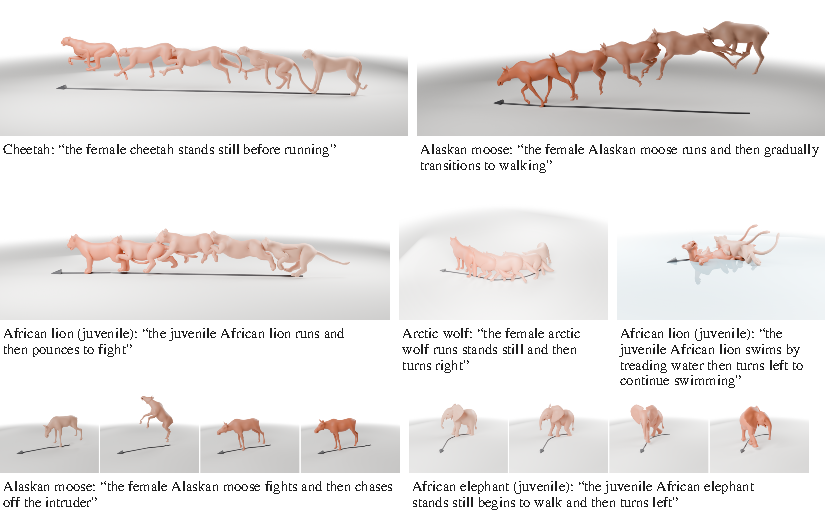
\includegraphics[width=0.9\linewidth]{figures/qualitative.pdf}
\caption{Seven generated clips of five library rigs on their production meshes. Travelling actions: four to
five poses at equal distances along the root path, light (first) to dark (last), with the root trajectory on the
ground. Actions on the spot: four frames at equal times from a fixed camera. Captions are the clips'
own.}\label{fig:qual}
\end{figure}

\subsection{Extending the model to rigs it has never seen}\label{sec:exp:extend}

\paragraph{Zero training and per-rig LoRA.} We take four Truebones rigs that differ from the
library in body plan and joint count -- Buffalo (30 joints), Gazelle (29), Dragon (95 joints, a
flying rig) and Spider (68) -- and compare three arms on the same held-out clips of each rig:
(a) the library model with the new rig's per-cell statistics, computed from all of its clips including
the evaluation clips, as its only rig-specific input (\emph{zero training}); (b) a per-rig
low-rank adapter trained on the rig's 8--26 training clips (\emph{LoRA}, \S\ref{sec:method:lora});
(c) a \num{36}M model of the same recipe trained on all \num{802} captioned Truebones clips,
evaluation clips included, as a seen-clip reference.
Table~\ref{tab:lora} gives the FK--pose gap on the held-out clips before and after adaptation next
to the articulation and jitter of the sampled output: eight to twenty-six clips bring the gap from
$0.25$--$1.2$ bone lengths to $0.08$--$0.15$, most on the two rigs farthest from the library, and
the seen-clip reference sits at $0.06$--$0.13$. Most of that is bought early: the jitter of the zero-training arm is
gone within 50--100 epochs and the gap plateaus by 150--200, after which longer adaptation changes nothing
(App.~\ref{app:extend_more}).

\begin{table}[t]
\centering\footnotesize\setlength{\tabcolsep}{3.5pt}
\caption{Extending \method{} (\num{303}M) to four Truebones rigs, each arriving with its own per-cell
statistics and masks. \emph{zero}: the library model served with those statistics and nothing
else --- articulation and jitter from that model, the gap from the adapter run's first validation, 10 to 15
steps in; \emph{LoRA}: the per-rig adapter; \emph{TB-only}: a \num{36}M model trained on all Truebones clips
including these. Gap in bone lengths; articulation and jitter of the sampled FK output relative to all real
clips of the rig (1 = real). App.~\ref{app:lora} and App.~\ref{app:extend_more} give the settings, the
\num{36}M study and a shared adapter for eight flying rigs.}\label{tab:lora}
\begin{tabular}{@{}llccccccccc@{}}
\toprule
& & \multicolumn{3}{c}{FK--pose gap (bl)$\downarrow$} & \multicolumn{3}{c}{Articulation ratio} & \multicolumn{3}{c}{Jitter ratio} \\
\cmidrule(lr){3-5}\cmidrule(lr){6-8}\cmidrule(lr){9-11}
Rig & Train / val & zero & LoRA & TB-only & zero & LoRA & TB-only & zero & LoRA & TB-only \\
\midrule
Buffalo (30 j.) & 15 / 5 & \num{0.323} & \num{0.132} & \num{0.072} & \num{1.45} & \num{0.30} & \num{0.67} & \num{3.32} & \num{0.33} & \num{1.02} \\
Gazelle (29 j.) & 8 / 2  & \num{0.255} & \num{0.084} & \num{0.062} & \num{5.39} & \num{0.77} & \num{1.22} & \num{13.2} & \num{0.86} & \num{1.92} \\
Dragon (95 j.)  & 10 / 3 & \num{1.215} & \num{0.146} & \num{0.134} & \num{1.02} & \num{0.49} & \num{1.23} & \num{2.53} & \num{0.52} & \num{1.12} \\
Spider (68 j.)  & 26 / 6 & \num{1.029} & \num{0.130} & \num{0.088} & \num{2.87} & \num{0.24} & \num{0.35} & \num{6.49} & \num{0.20} & \num{0.37} \\
\bottomrule
\end{tabular}
\end{table}

\subsection{Relation to prior work}\label{sec:exp:compare}

\paragraph{Capabilities.} The two capabilities this paper joins are available separately in released
systems (Table~\ref{tab:open}): those that take the kinematic tree at inference are not text-conditioned, and
the text-conditioned animal generators are built around one fixed skeleton. \method{} returns rotations and a
world-space root trajectory the rig plays as generated, and measures that geometry against ground truth for the
pilot and the main model alike (Table~\ref{tab:physical}: at \num{303}M the FK--pose gap is \num{0.24} bone
lengths, the foot slide \num{1.84} against a real \num{2.03}). Table~\ref{tab:capability} adds the systems whose
code is not public. The construction those systems reach a second skeleton with --- every joint padded into one
flat per-frame vector --- is trained on our corpus at our budget in App.~\ref{app:flat} and read beside the
ablations in Table~\ref{tab:simple}.

\begin{table}[t]
\centering\footnotesize\setlength{\tabcolsep}{4pt}
\caption{Systems with a public implementation we could run. \emph{Topology}: the kinematic tree is an input at
inference, not fixed by the architecture. \emph{Rotations} / \emph{Root}: joint rotations and a world-space root
trajectory, not positions a solver must turn back into a pose.}\label{tab:open}
\begin{tabular}{@{}lccccc@{}}
\toprule
System & Code & Text & Topology & Rotations & Root \\
\midrule
Human T2M~\citep{tevet2023mdm,zhang2024motiondiffuse} & $\checkmark$ & $\checkmark$ & $\times$ & $\checkmark$ & $\checkmark$ \\
Animal T2M~\citep{wang2025animo,yang2024omnimotiongpt} & $\checkmark$ & $\checkmark$ & $\times$ & $\checkmark$ & $\checkmark$ \\
AnyTop~\citep{gat2025anytop} & $\checkmark$ & $\times$ & $\checkmark$ & $\checkmark$ & $\checkmark$ \\
\method{} (ours) & --- & $\checkmark$ & $\checkmark$ & $\checkmark$ & $\checkmark$ \\
\bottomrule
\end{tabular}
\end{table}


\paragraph{AnyTop as an in-distribution reference.} The released AnyTop weights trained on the whole
Truebones zoo, including the four rigs of Table~\ref{tab:lora}, so its per-rig geometry
(App.~\ref{app:anytop}) is a reference for what a model trained on these rigs produces.

\subsection{Ablations}\label{sec:exp:ablation}

The ablations share the pilot's recipe and checkpoint epoch; App.~\ref{app:ablation_notes} collects them
with the notes. Flattening the joint axis into one token per frame --- the construction that carries a
fixed-skeleton generator to variable skeletons --- costs \num{0.198}--\num{0.208} of R@1 and multiplies the FID
by \num{3.7}, with the corpus, split, captions, rest pose, objective, weights, schedule and budget matched and
\num{5}\% more parameters on the flat side (Table~\ref{tab:simple}, App.~\ref{app:flat}). Keeping the joint
axis and removing what this paper puts on it costs \num{0.067}--\num{0.072}, of which the calibrated group
weights carry \num{0.036}--\num{0.045}, the geodesic and direction biases and the structural features
\num{0.028}--\num{0.035}, and the joint descriptions none. The acceleration-matching
term changes nothing (Table~\ref{tab:ablation}). Per-cell mean and standard deviation are worth about two points of R@1 over a per-rig scale alone and \num{22}--\num{30}\% of the FID at every matched
epoch (Table~\ref{tab:rep}). Its channel layout is worth under a point of R@1 against the 13-channel AnyTop
layout derived from the same clips (Table~\ref{tab:repcontent}), and \num{0.007} once that arm's own objective
and partition are matched, so retrieval is measuring the objective rather than the layout; what the layout does
change is the leaf articulation, foot contact and root travel of Table~\ref{tab:physical}, and the agreement of
the two output channels --- re-encoding a sample through the forward kinematics of its own rotations costs
\num{0.005} of R@1 on \rep{} against \num{0.035} on the 13-channel layout (Table~\ref{tab:controls}). At a
matched budget of 200 epochs the \num{36}M, \num{116}M and \num{303}M models reach R@1 \num{0.878},
\num{0.900} and \num{0.914} (Table~\ref{tab:size}).

